\section{TODO}
   	\subsection{Grundelemente}
   	\begin{tabular}{p{1.5cm} p{4.3cm} |p{1.5cm} p{4.3cm}| p{1.5cm} p{4.3cm}}
   		\multicolumn{2}{l}{\textbf{Ohmscher Widerstand R}}
   		& \multicolumn{2}{l}{\textbf{Kapazitität C}}
   		& \multicolumn{2}{l}{\textbf{Induktivität L}} \\
   		\multicolumn{2}{l}{$u$ und $i$ können sprunghaft ändern}
   		& \multicolumn{2}{l}{$\mathbf{u}$ \textbf{kann nicht sprunghaft ändern}}
   		& \multicolumn{2}{l}{$\mathbf{i}$ \textbf{kann nicht sprunghaft ändern}} \\
   		
   		\multirow{2}{1.5cm}{
   			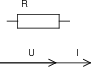
\includegraphics[width=1.5cm]{./images/zeigerdiag-r.png}}
   		& $u(t) = R \cdot i(t)$ 
   		& \multirow{2}{1.5cm}{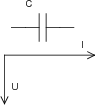
\includegraphics[width=1.5cm]{./images/zeigerdiag-c.png}}
   		& $u(t) = \frac{1}{C} \int\limits_0^t i(\tau) d\tau + u(0)$
   		& 
   		\multirow{2}{1.5cm}{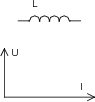
\includegraphics[width=1.5cm]{./images/zeigerdiag-l.png}}
   		&$u(t) = L \frac{di(t)}{dt}$\\
   		
   		&$i(t) = \frac{u(t)}{R}$
   		& & $i(t) = C \frac{d u(t)}{dt}$
   		& & $i(t) = \frac{1}{L} \int\limits_0^t u(\tau) d\tau + i(0)$\\
   		
   		& $\underline{Z}_R = R$
   		& & $\underline{Z}_C = \frac{1}{j \omega C} = - \frac{j}{\omega C}$
   		& & $\underline{Z_L} = j \omega L$\\
   		
   		\parbox{1.7cm}{\small{nicht linear:}}
   		& $R_=(u) = \frac{U}{I(u)}, r_D = \frac{\diff U}{\diff I}\lvert_{U_0}$
   		& & $X_C = -\frac{1}{\omega C} \quad B_C = \omega C$
   		& & $X_L = \omega L
   		\quad B_L = -\frac{1}{\omega L}$ \\
   		
   		& $P=I^2 \cdot R = \frac{U^2}{R}$
   		& & $Q_C= - U^2 \cdot \omega C = - \frac{I^2}{\omega C}$
   		& & $Q_L= I^2 \cdot \omega L = \frac{U^2}{\omega L}$\\
   		
   		& & & $W_C=\frac12 C U_C^2$
   		& &$W_L=\frac12 L I_L^2$
   	\end{tabular}

	\subsection{Begriffe der Impedanz und Admitanz}
	\begin{tabular}{lllll}
		Scheinwiderstand & & $Z = \frac{U_{eff}}{I_{eff}} $ & $ =
		\sqrt{R^2+X^2}$ & Ohm\\ Komplexer Widerstand & Impedanz & $\underline Z = R + jX = Z \cdot e^{j \varphi}$ 
		& $  = \dfrac{\underline{U}}{\underline{I}} = \dfrac{\underline{U}\cdot\underline{U}^{\ast}}{\underline{S}^*} =  = \dfrac{U^2}{\underline{S}^*} = 
		\dfrac{\underline{S}}{I^2}$ & Ohm\\
		Komplexer Leitwert & Admittanz & $\underline Y = G + jB =
		\frac{1}{\underline Z} = \frac{1}{Z}e^{-j\varphi}$ & $= \frac{\underline{I}}{\underline{U}}$ &  Siemens\\
		Wirkwiderstand & Resistanz & $R = \Real(\underline Z) $ & $ = Z
		\cdot cos(\varphi)$ & Ohm\\
		Wirkleitwert & Konduktanz & $G = \Real(\underline Y) $ & $ \neq \frac{1}{R}$ &
		Siemens\\
		Blindwiderstand & Reaktanz & $X = \Imag(\underline Z) $ & $ = Z
		\cdot sin(\varphi)$ & Ohm\\
		Blindleitwert & Suszeptanz & $B = \Imag( \underline Y) $ & $ \neq \frac{1}{X}$
		& Siemens\\
		Phasenverschiebung & & $\varphi = \varphi_u - \varphi_i =
		\arctan\left(\frac{\Imag(\underline{Z})}{\Real(\underline{Z})}\right)$ & &
		Radiant\\
		
	\end{tabular}
		
	\subsection{Formeln Übung 5}
    \begin{tabular}[b]{|C{4cm}| P{8cm} | P{5cm}|}
        \hline
        \textbf{Polradwinkel}&
        \[ p(\delta)=\frac{U_p \cdot U_1}{X_d} sin(\delta) \]&
        $ \delta$ = Polradwinkel \newline
        $ U_p = $ Polradspannung \newline
        $ L_d =$ Synchroninduktivität (?)
        \\ \hline
        
        \textbf{Polpaarzahl}&
        $ p=\frac{60 \cdot f}{n} $&
        $ \left[n= \frac{1}{min}\right] $
        \\ \hline
        
        &
        \[  \frac{sin(\delta)}{2\pi f L_d}=\frac{sin(\delta ')}{2\pi f L_d '} \] &
        \\ \hline       
    \end{tabular}
    \clearpage
    \pagebreak

    \subsection{V11-12 S43}
        \begin{longtable}{| p{.40\textwidth} | p{.60\textwidth} |}
             \firsthline
              \newline
              \tabbild[scale=0.6]{images/StatordqSM1}&
              $ \varPhi_m(y_r,i) = L(y_r(t)) \cdot i(t) $\newline
              \[ u_{Statorkreis}(t)=R\cdot i(t) + \frac{\diff\varPhi_m}{\diff t}(t) = R \cdot i(t) + \frac{\diff}{\diff t}\left[L(y_r(t))\cdot i(t) \right]\] 
              \[\qquad = R \cdot i(t) + \frac{\diff L}{\diff  y_r} (y_r)\cdot \frac{\diff  y_r}{\diff t} i(t) +L(y_r)\cdot \frac{\diff i}{\diff t}(t)\]
              \[ p_{Statorkreis}(t)=u(t) \cdot i(t) = R\cdot i^2(t)+\frac{\diff L}{\diff Y_r}(y_r)\cdot \omega_r\cdot i^2(t)+L\cdot i(t)\cdot \frac{\diff i}{\diff t}(t) \]
              \\ \hline
              
              \textbf{Elektrische Leistung des Stators}&
              \[ p(t) = R \cdot i^2(t) + \frac{\diff L}{\diff y_r}\cdot \omega_r \cdot i^2(t) + L \cdot i(t) \cdot\frac{\diff i}{\diff t}(t) \]
              \[=p_{Cu}(t)+\frac{\diff w_m}{\diff t}(t)+\frac{1}{2}\cdot \frac{\diff L}{\diff y_r}(y_r)\cdot \omega_r \cdot i^2(t) \]
              \\ \hline
              
              \textbf{Zeitableitung magnetischer Energie}&
              \[ w_m(t) = \frac{1}{2} \cdot L(y_r) \cdot i^2(t) \Rightarrow \frac{\diff }{\diff t} \left( \frac{1}{2} \cdot L(y_r) \cdot i^2(t) \right) \]
              \[=\frac{1}{2}\cdot \frac{\diff L}{\diff y_r}(y_r)\cdot\omega_r \cdot i^2(t) + L \cdot i(t) \cdot \frac{\diff i}{\diff t}(t) \]
              \\ \hline
              
              \textbf{Rotorleistung}&
              \[ p_\delta(t)= \frac{1}{2}\cdot \frac{\diff L}{\diff y_r}(y_r)\cdot \omega_r \cdot i^2(t) \]
              \\ \hline
              
              \textbf{Motormoment}&
              \[ m_M(t)=\frac{p_\delta}{\omega_r}(t)=\frac{1}{2}\cdot\frac{\diff L}{\diff y_r}(y_r)\cdot i^2(t) \]
              \\ \hline
              
               \newline
              \tabbild[scale=0.7]{images/IndukdqSMY}&
               \newline
              \tabbild[scale=0.7]{images/MomentdqSMY}
              \\ \hline
              
              \textbf{Betriebsverhalten}\newline
              \[ J_g \frac{\diff \omega_r}{\diff t}= J_g \frac{\omega_s - \omega_1}{T_s} = M_M - M_L \] \newline
               $ \omega_s = 2\pi\frac{n_s}{60}=2\pi\frac{f_s}{N_p}=\alpha_0 f_s $&
              $ J_g $ = Motorbezogenes Trägheitsmoment \newline
              $ M_M $ = Motorbezogenes Drehmoment \newline
              $ M_L $ = Lastmoment \newline
              $ \omega_s $ = Kreisgeschwindigkeit Statorfeld \newline
              $ \omega_1 $ = Kreisgeschwindigkeit des Rotors \newline
              $\Rightarrow  \omega_1 = 0 \Rightarrow$ Motor im Stillstand \newline
              \\ \hline
              
              \textbf{Lastmoment} \newline
              \[ M_L(f_s,\omega_1) = M_M -J_g\frac{\omega_s}{T_s}+J_g\frac{\omega_1}{T_s}\]
              \[=M_m -J_g\alpha_0F_s^2+J_g\omega_1f_s \]&
              \newline
              $ F_s = \frac{1}{T_s} $ = Schaltfrequenz\newline
              $ \omega_1 $ = Anfangsgeschwindigkeit \newline
              \\ \hline
              
              \textbf{Anlaufkennlinie}\newline
              \tabbild[scale=0.4]{images/AnlaufkennlinieSM.JPG}&
              $ f_{AG} $ = Anlaufgrenzfrequenz \newline
              $ f_{BG} $ =  Betriebsgrenzfrequenz
              \\ \hline
              
              
              
              
              
              
              
        \end{longtable}
